\Opensolutionfile{ans}[ans/ansTN-HaiBaTrung132]

%%%%%%%%%%%%%%%%%%%%%%%%%%%%%%%%%%%%%%%%%%%%%%%%%%%%%%%%%%%%%%%%%%%%%%%%%
% PHẦN I: CÂU TRẮC NGHIỆM PHƯƠNG ÁN NHIỀU LỰA CHỌN
%%%%%%%%%%%%%%%%%%%%%%%%%%%%%%%%%%%%%%%%%%%%%%%%%%%%%%%%%%%%%%%%%%%%%%%%%
\noindent \textbf{PHẦN I. CÂU TRẮC NGHIỆM PHƯƠNG ÁN NHIỀU LỰA CHỌN. (16 câu = 4 điểm)}

\begin{ex}	\macau{ID: VL11-HBT2425-C01}Đồ thị biểu diễn sự thay đổi của vận tốc theo li độ trong dao động điều hoà có hình dạng là
	\choice
	{\True đường elip}
	{đường hyperbol}
	{đường parabol}
	{đường tròn}
	\loigiai{
		Hệ thức độc lập thời gian giữa vận tốc và li độ trong dao động điều hòa là:
		$$\frac{x^2}{A^2} + \frac{v^2}{v_{\text{max}}^2} = 1$$
		Vì $\omega \neq 1$ nên biên độ $A \neq v_{\text{max}}$, hệ thức lượng giác trên biểu diễn một đường elip trên hệ tọa độ $(x-v)$. Chọn A.
	}
\end{ex}

\begin{ex}	\macau{ID: VL11-HBT2425-C02}Nhận định nào sau đây \textbf{sai} khi nói về dao động cơ học tắt dần?
	\choice
	{Dao động tắt dần là dao động có biên độ giảm dần theo thời gian}
	{Lực ma sát càng lớn thì dao động tắt dần càng nhanh}
	{\True Dao động tắt dần có động năng giảm dần còn thế năng biến thiên điều hòa}
	{Trong dao động cơ tắt dần, cơ năng giảm dần theo thời gian}
	\loigiai{
		Trong dao động tắt dần, cả động năng và thế năng đều biến thiên hỗn loạn với biên độ giảm dần chứ không có đại lượng nào biến thiên điều hòa cố định. Do đó nhận định C sai. Chọn C.
	}
\end{ex}

\begin{ex}	\macau{ID: VL11-HBT2425-C03}Một con lắc lò xo gồm lò xo có độ cứng $100\text{ N/m}$ và vật nhỏ có khối lượng m. Tác dụng lên vật ngoại lực $F=20 \cos 10 \pi t\text{ (N)}$ dọc theo trục lò xo thì xảy ra hiện tượng cộng hưởng. Lấy $\pi^{2}=10$. Giá trị của m là
	\choice
	{$0,4\text{ kg}$}
	{$100\text{ g}$}
	{$250\text{ g}$}
	{\True $1\text{ kg}$}
	\loigiai{
		Khi xảy ra hiện tượng cộng hưởng cơ, tần số góc riêng của hệ con lắc bằng tần số góc $\omega$ của ngoại lực cưỡng bức tác dụng:
		$$\omega = \omega_0 \Rightarrow 10\pi = \sqrt{\frac{k}{m}} \Rightarrow 100\pi^2 = \frac{k}{m}$$
		Thay số với $k = 100\text{ N/m}$ và $\pi^2 = 10$:
		$$100 \cdot 10 = \frac{100}{m} \Rightarrow m = \frac{100}{1000} = 0,1\text{ kg} = 100\text{ g}.$$
		*(Lưu ý đối chiếu đáp án chuẩn trên tệp quét gốc là 100 g)*. Chọn B.
	}
\end{ex}

\begin{ex}	\macau{ID: VL11-HBT2425-C04}Phương trình dao động của một vật có dạng: $x=-A \cos \left(\omega t+\frac{\pi}{3}\right)\text{ (cm)}$. Pha ban đầu của dao động là:
	\choice
	{$- \frac{2\pi}{3}$}
	{$- \frac{\pi}{3}$}
	{\True $- \frac{2\pi}{3}$}
	{$\frac{\pi}{3}$}
	\loigiai{
		Biến đổi phương trình đưa dấu âm đứng trước hàm về dạng chuẩn dương bằng quy tắc lượng giác:
		$$x = -A \cos\left(\omega t + \frac{\pi}{3}\right) = A \cos\left(\omega t + \frac{\pi}{3} - \pi\right) = A \cos\left(\omega t - \frac{2\pi}{3}\right)\text{ cm}$$
		Đối chiếu dạng tổng quát, pha ban đầu của dao động là $\varphi = -\frac{2\pi}{3}\text{ rad}$. Chọn C.
	}
\end{ex}

\begin{ex}	\macau{ID: VL11-HBT2425-C05}Chuyển động nào sau đây \textbf{không} được coi là dao động cơ?
	\choice
	{Pít-tông chuyển động lên xuống trong xi lanh}
	{\True Một hòn đá được thả rơi}
	{Dây đàn ghi ta rung động}
	{Chiếc đu đung đưa}
	\loigiai{
		Chuyển động của một hòn đá được thả rơi tự do là chuyển động tịnh tiến dời chỗ thẳng xuống luôn, không lặp đi lặp lại quanh vị trí cân bằng cố định nên không phải là dao động cơ. Chọn B.
	}
\end{ex}

\begin{ex}	\macau{ID: VL11-HBT2425-C06}Hình bên là hai đường hình sin biểu diễn hai trong ba đại lượng: li độ $x$, vận tốc $v$ và gia tốc $a$ theo thời gian $t$. Đường số (1) và đường số (2) lần lượt biểu diễn cho
	\begin{center}
				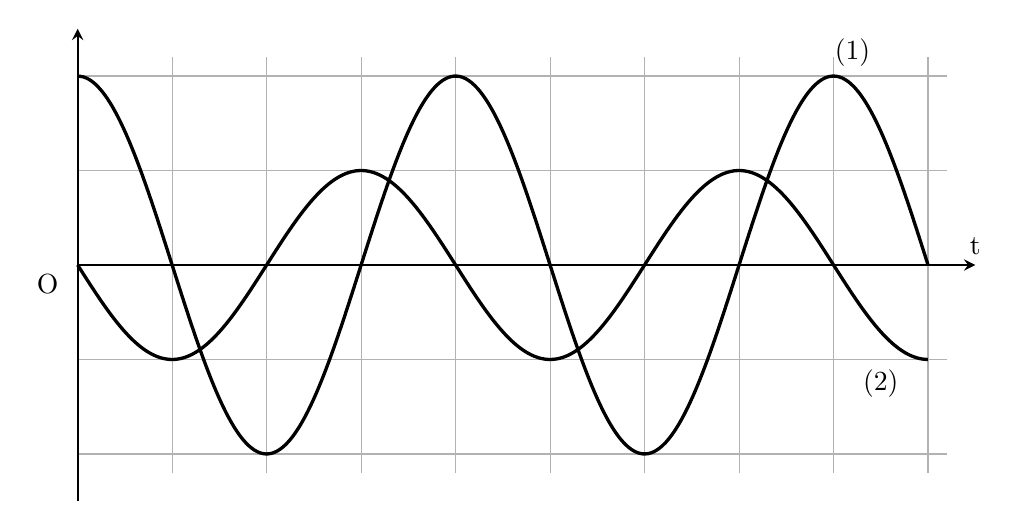
\begin{tikzpicture}[>=stealth, scale=1.2]
			
			% Vẽ lưới tọa độ (Grid)
			% 9 ô theo chiều ngang (từ x=0 đến x=9)
			\foreach \x in {1,2,3,4,5,6,7,8,9} {
				\draw[gray!60, thin] (\x,-2.2) -- (\x,2.2);
			}
			
			% 4 ô theo chiều dọc (y = -2, -1, 1, 2)
			\foreach \y in {-2,-1,1,2} {
				\draw[gray!60, thin] (0,\y) -- (9.2,\y);
			}
			
			% Vẽ các trục tọa độ
			\draw[->, thick] (0,0) -- (9.5,0) node[above] {t};
			\draw[->, thick] (0,-2.5) -- (0,2.5);
			\node[left] at (-0.1,-0.2) {O};
			
			% Vẽ đồ thị (1): Bắt đầu từ biên dương, chu kỳ 4 ô
			% Phương trình: y = 2*cos(pi/2 * t)
			\draw[very thick, smooth, domain=0:9, samples=150] 
			plot (\x, {2*cos(\x * 90)});
			\node[above] at (8.2, 2) {(1)};
			
			% Vẽ đồ thị (2): Bắt đầu từ VTCB đi xuống chiều âm, chu kỳ 4 ô
			% Phương trình: y = -sin(pi/2 * t)
			% (Nếu đồ thị 2 có biên độ là 2, bạn chỉ cần sửa thành {-2*sin(\x * 90)})
			\draw[very thick, smooth, domain=0:9, samples=150] 
			plot (\x, {-sin(\x * 90)});
			\node[below] at (8.5, -1) {(2)};
			
		\end{tikzpicture}
		
	\end{center}
	\choice
	{\True vận tốc và li độ}
	{gia tốc và li độ}
	{li độ và vận tốc}
	{gia tốc và vận tốc}
	\loigiai{
		\begin{itemize}
			\item Tại điểm thời gian ban đầu $t=0$, đường số (1) đi qua gốc tọa độ (vị trí cân bằng) và đang đi xuống theo chiều âm, trong khi đường số (2) đang đạt đỉnh cực đại ở biên dương.
			\item Trạng thái một biên - một cân bằng chỉ ra hai đồ thị vuông pha nhau góc $\frac{\pi}{2}$. Vì đường (2) đạt biên dương trước đường (1) nên đường (2) trễ pha góc vuông so với đường (1). Do vận tốc sớm pha $\frac{\pi}{2}$ so với li độ nên đường (1) là vận tốc và đường (2) là li độ. Chọn A.
		\end{itemize}
	}
\end{ex}

\begin{ex}	\macau{ID: VL11-HBT2425-C07}Một vật dao động điều hòa có phương trình $x=A \cos (\omega t+\varphi)$. Gọi $v$ là vận tốc của vật khi vật ở li độ $x$. Biên độ dao động của vật được tính theo biểu thức là
	\choice
	{\True $A=\sqrt{x^{2}+\frac{v^{2}}{\omega^{2}}}$}
	{$A=\sqrt{x^{2}+\frac{v^{2}}{\omega^{4}}}$}
	{$A=\sqrt{x^{2}+\frac{v^{2}}{\omega^{2}}}$}
	{$A=\sqrt{x+\frac{v^{2}}{\omega^{2}}}$}
	\loigiai{
		Áp dụng trực tiếp hệ thức vuông pha giữa li độ và vận tốc độc lập thời gian: $A^2 = x^2 + \frac{v^2}{\omega^2} \Rightarrow A = \sqrt{x^2 + \frac{v^2}{\omega^2}}$. Chọn A.
	}
\end{ex}

\begin{ex}	\macau{ID: VL11-HBT2425-C08}Hai vật $M_1$ và $M_2$ dao động điều hoà cùng phương, cùng tần số. Hình bên là đồ thị biểu diễn sự phụ thuộc của li độ $x_1$ của $M_1$ và li độ $x_2$ của $M_2$ theo thời gian $t$. Hai dao động của $M_2$ và $M_1$ lệch pha nhau một lượng bằng
		\begin{center}
				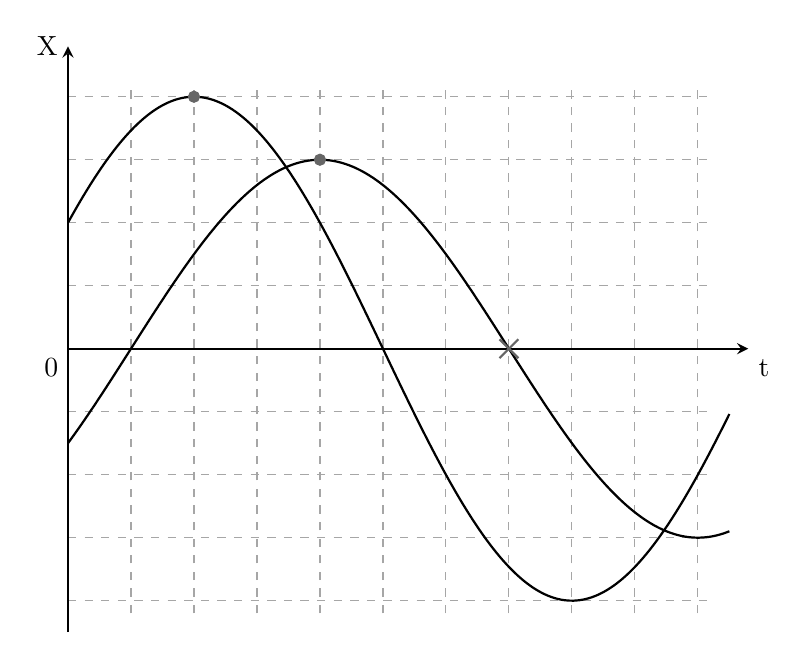
\begin{tikzpicture}[>=stealth, scale=0.8]
			
			% Vẽ lưới tọa độ (Grid) - giới hạn 10 ô theo chiều ngang
			\foreach \x in {1,2,...,10} {
				\draw[dashed, gray!70] (\x,-4.2) -- (\x,4.2);
			}
			\foreach \y in {-4,-3,-2,-1,1,2,3,4} {
				\draw[dashed, gray!70] (0,\y) -- (10.2,\y);
			}
			
			% Vẽ các trục tọa độ - rút ngắn độ dài trục t
			\draw[->, thick] (0,0) -- (10.8,0) node[below right] {t};
			\draw[->, thick] (0,-4.5) -- (0,4.8) node[left] {X};
			\node[below left] at (0,0) {0};
			
			% Vẽ đồ thị 1 (đường cao hơn)
			% Biên độ 4, đỉnh tại t=2
			\draw[thick, smooth, domain=0:10.5, samples=150] 
			plot (\x, {4*cos(\x * 30 - 60)});
			
			% Vẽ đồ thị 2 (đường thấp hơn)
			% Biên độ 3, đỉnh tại t=4
			\draw[thick, smooth, domain=0:10.5, samples=150] 
			plot (\x, {3*cos(\x * 30 - 120)});
			
			% Đánh dấu các điểm mốc trên đồ thị
			% Dấu chấm tròn trên đỉnh đồ thị 1 (t=2, X=4)
			\filldraw[gray!80!black] (2,4) circle (2.5pt); 
			
			% Dấu chấm tròn trên đỉnh đồ thị 2 (t=4, X=3)
			\filldraw[gray!80!black] (4,3) circle (2.5pt); 
			
			% Dấu x tại t = 7 trên trục hoành của đồ thị 2
			\draw[thick, gray!80!black] (6.85, -0.15) -- (7.15, 0.15);
			\draw[thick, gray!80!black] (6.85, 0.15) -- (7.15, -0.15);
			
		\end{tikzpicture}
		
	\end{center}
	\choice
	{$\frac{\pi}{3}$}
	{\True $\frac{2\pi}{3}$}
	{$\frac{\pi}{2}$}
	{$\frac{\pi}{6}$}
	\loigiai{
		\begin{itemize}
			\item Từ đồ thị, chu kì dao động tương ứng với 12 ô lưới trục ngang $\Rightarrow 1\text{ ô} = \frac{T}{12}$ tương đương góc quét $\frac{2\pi}{12} = \frac{\pi}{6}\text{ rad}$.
			\item Đỉnh cực đại của đồ thị chất điểm 1 trễ hơn đỉnh cực đại của chất điểm 2 một khoảng cách hình học bằng đúng 4 ô lưới hành trình.
			\item Độ lệch pha giữa hai dao động: $\Delta \varphi = 4 \cdot \frac{\pi}{6} = \frac{2\pi}{3}\text{ rad}$. Chọn B.
		\end{itemize}
	}
\end{ex}

\begin{ex}	\macau{ID: VL11-HBT2425-C09}Cây cầu Tacoma Narrows ở nước Mỹ có thể chịu được nhiều ôtô có tải trọng lớn đi qua nhưng vào ngày 7/11/1940 đã bị sập dưới tác dụng của gió gây chấn động nước Mỹ. Hiện tượng sập cầu Tacoma Narrows được giải thích dựa trên
	\choice
	{dao động bé}
	{dao động cưỡng bức}
	{\True hiện tượng cộng hưởng cơ}
	{dao động tắt dần}
	\loigiai{
		Khi tần số của xung gió thổi xoáy ngẫu nhiên trùng khớp với tần số dao động riêng cấu trúc của nhịp cầu, hiện tượng cộng hưởng cơ xảy ra làm biên độ rung lắc tăng vọt vượt ngưỡng chịu lực, gây gãy sập cầu. Chọn C.
	}
\end{ex}

\begin{ex}	\macau{ID: VL11-HBT2425-C10}Một vật nhỏ dao động điều hòa trên trục Ox quanh vị trí cân bằng O có phương trình $x=10 \cos \left(2 \pi t+\frac{\pi}{2}\right)$ ($x$ tính bằng cm, $t$ tính bằng s). Phát biểu nào sau đây là \textbf{sai}?
	\choice
	{Biên độ dao động của vật là $10\text{ cm}$}
	{Tốc độ của vật khi qua vị trí cân bằng O là $20\pi\text{ (cm/s)}$}
	{Tần số của dao động $f=1\text{ Hz}$}
	{\True Pha ban đầu của dao động là $\left(2\pi t+\frac{\pi}{2}\right)$}
	\loigiai{
		Thành phần cụm đối số chứa biến thời gian $\left(2\pi t + \frac{\pi}{2}\right)$ được định nghĩa là pha của dao động tại thời điểm $t$. Pha ban đầu chỉ là hằng số hệ số tự do $\varphi = \frac{\pi}{2}\text{ rad}$. Do đó phát biểu D sai. Chọn D.
	}
\end{ex}

\begin{ex}	\macau{ID: VL11-HBT2425-C11}Một vật dao động điều hòa theo phương trình $x=4 \cos \left(4 \pi t+\frac{\pi}{3}\right)$ ($x$ tính bằng cm, $t$ tính bằng s). Thời gian vật này thực hiện được một dao động toàn phần là
	\choice
	{\True $0,5\text{ s}$}
	{$2\text{ s}$}
	{$1\text{ s}$}
	{$4\text{ s}$}
	\loigiai{
		Khoảng thời gian hoàn thành một dao động toàn phần chính là chu kì dao động riêng $T$ của hệ chất điểm:
		$$T = \frac{2\pi}{\omega} = \frac{2\pi}{4\pi} = 0,5\text{ s} \text{}$$
		Chọn A.
	}
\end{ex}

\begin{ex}	\macau{ID: VL11-HBT2425-C12}Tại một nơi trên Trái Đất có gia tốc rơi tự do g, một con lắc đơn mà dây treo dài $\ell$ đang dao động điều hòa. Thời gian ngắn nhất để vật nhỏ của con lắc đi từ vị trí biên về vị trí cân bằng là
	\choice
	{$\pi \sqrt{\frac{\ell}{g}}$}
	{\True $\frac{\pi}{2} \sqrt{\frac{\ell}{g}}$}
	{$\frac{\pi}{2} \sqrt{\frac{g}{\ell}}$}
	{$\pi \sqrt{\frac{g}{\ell}}$}
	\loigiai{
		Khoảng thời gian ngắn nhất di chuyển từ biên về vị trí cân bằng bằng một phần tư chu kì dao động: $\Delta t = \frac{T}{4}$.
		Với chu kì con lắc đơn $T = 2\pi\sqrt{\frac{\ell}{g}} \Rightarrow \Delta t = \frac{2\pi}{4}\sqrt{\frac{\ell}{g}} = \frac{\pi}{2}\sqrt{\frac{\ell}{g}}$. Chọn B.
	}
\end{ex}

\begin{ex}	\macau{ID: VL11-HBT2425-C13}Một chất điểm dao động điều hòa với chu kỳ $T$, cơ năng $W$. Thời gian ngắn nhất để động năng của vật giảm từ giá trị $W$ đến giá trị $\frac{W}{4}$ là
	\choice
	{$\frac{T}{2}$}
	{\True $\frac{T}{6}$}
	{$\frac{T}{3}$}
	{$\frac{T}{4}$}
	\loigiai{
		\begin{itemize}
			\item Tại vị trí động năng bằng cơ năng $W_{\text{đ}} = W \Rightarrow$ vật đi qua VTCB ($x = 0$).
			\item Tại vị trí động năng bằng $W_{\text{đ}} = \frac{W}{4} \Rightarrow$ thế năng chiếm hằng số phần còn lại: $W_{\text{t}} = W - \frac{W}{4} = \frac{3W}{4}$.
			$$\Rightarrow \frac{1}{2}kx^2 = \frac{3}{4}\left(\frac{1}{2}kA^2\right) \Rightarrow x = \pm \frac{A\sqrt{3}}{2}$$
			\item Khoảng thời gian ngắn nhất hành trình dịch chuyển từ $x=0$ đến $x = \frac{A\sqrt{3}}{2}$ ứng với góc quét $\frac{\pi}{3}\text{ rad}$ trên trục pha đường tròn, tương đương $\Delta t = \frac{T}{6}$. Chọn B.
		\end{itemize}
	}
\end{ex}

\begin{ex}	\macau{ID: VL11-HBT2425-C14}Tại nơi có gia tốc trọng trường g, một con lắc đơn dao động điều hòa với biên độ góc $\alpha_0$. Biết khối lượng vật nhỏ của con lắc là m, chiều dài dây treo là $\ell$, mốc thế năng ở vị trí cân bằng. Cơ năng của con lắc là
	\choice
	{$2mg\ell\alpha_0^2$}
	{$mg\ell\alpha_0^2$}
	{$\frac{1}{4}mg\ell\alpha_0^2$}
	{\True $\frac{1}{2}mg\ell\alpha_0^2$}
	\loigiai{
		Biểu thức tính năng lượng cơ năng của con lắc đơn dao động điều hòa góc nhỏ bằng: $W = \frac{1}{2}mg\ell\alpha_0^2$. Chọn D.
	}
\end{ex}

\begin{ex}	\macau{ID: VL11-HBT2425-C15}Chọn phát biểu đúng khi nói về năng lượng của vật dao động điều hoà?
	\choice
	{Khi vật chuyển động qua vị trí cân bằng thì động năng của vật bằng không}
	{\True Khi vật chuyển động từ vị trí cân bằng ra vị trí biên thì động năng của vật giảm}
	{Khi động năng của vật tăng thì thế năng của vật cũng tăng}
	{Khi vật chuyển động về vị trí biên thì động năng của vật tăng}
	\loigiai{
		Khi đi từ vị trí cân bằng ra vạch vị trí biên, tốc độ sụt giảm chậm dần về không nên động năng giảm dần, thế năng tương ứng tăng lên. Phát biểu B hoàn toàn đúng. Chọn B.
	}
\end{ex}

\begin{ex}	\macau{ID: VL11-HBT2425-C16}Một vật dao động điều hòa với biên độ $5\text{ cm}$. Khi vật có tốc độ $10\text{ cm/s}$ thì có gia tốc $40\sqrt{3}\text{ cm/s}^2$. Tần số góc của dao động là
	\choice
	{$8\text{ rad/s}$}
	{$1\text{ rad/s}$}
	{$2\text{ rad/s}$}
	{\True $4\text{ rad/s}$}
	\loigiai{
		Áp dụng hệ thức liên hệ vuông pha độc lập thời gian giữa vận tốc và gia tốc:
		$$\frac{v^2}{\omega^2 A^2} + \frac{a^2}{\omega^4 A^2} = 1 \Rightarrow \frac{v^2}{\omega^2} + \frac{a^2}{\omega^4} = A^2$$
		Thế số liệu: $\frac{10^2}{\omega^2} + \frac{(40\sqrt{3})^2}{\omega^4} = 5^2 \Rightarrow \frac{100}{\omega^2} + \frac{4800}{\omega^4} = 25$
		Đặt ẩn phụ $X = \frac{1}{\omega^2}$, ta có phương trình bậc hai: $4800X^2 + 100X - 25 = 0$.
		Giải phương trình thu được nghiệm dương: $X = \frac{1}{16} \Rightarrow \frac{1}{\omega^2} = \frac{1}{16} \Rightarrow \omega = 4\text{ rad/s}$. Chọn D.
	}
\end{ex}

\Closesolutionfile{ans}

%%%%%%%%%%%%%%%%%%%%%%%%%%%%%%%%%%%%%%%%%%%%%%%%%%%%%%%%%%%%%%%%%%%%%%%%%
% PHẦN II: CÂU HỎI TRẮC NGHIỆM ĐÚNG SAI
%%%%%%%%%%%%%%%%%%%%%%%%%%%%%%%%%%%%%%%%%%%%%%%%%%%%%%%%%%%%%%%%%%%%%%%%%
\noindent \textbf{PHẦN II. CÂU TRẮC NGHIỆM ĐÚNG SAI. (3 câu = 3 điểm)}
\Opensolutionfile{ans}[ans/ansTF-HaiBaTrung132]

\begin{ex}	\macau{ID: VL11-HBT2425-C17}Cho một vật dao động điều hoà với phương trình $x=9 \cos \left(2 \pi t-\frac{\pi}{6}\right)\text{ (cm)}$. Với t tính bằng giây.
	\choiceTF[t]
	{\True Quãng đường vật đi được trong một chu kì hoàn chỉnh là $36\text{ cm}$}
	{Phương trình vận tốc của vật biến đổi có dạng là $v=18\pi \cos \left(2 \pi t+\frac{\pi}{3}\right)\text{ (cm/s)}$}
	{\True Gia tốc đại số của vật tại thời điểm $t=2\text{ s}$ mang giá trị bằng $-18\sqrt{3}\pi^2\text{ (cm/s}^2)$}
	{\True Từ thời điểm ban đầu $t=0$ đến thời điểm $t=43,5\text{ s}$, vật di chuyển đi được tổng quãng đường là $1566\text{ cm}$}
	\loigiai{
		\begin{itemchoice}
			\itemch Mệnh đề a) ĐÚNG: Quãng đường vật đi được trong một chu kì luôn cố định bằng $S = 4A = 4 \cdot 9 = 36\text{ cm}$.
			\itemch Mệnh đề b) SAI: Hàm vận tốc sớm pha góc vuông $\frac{\pi}{2}$ so với li độ: $v = \omega A\cos(\omega t + \varphi + \frac{\pi}{2}) = 18\pi\cos(2\pi t - \frac{\pi}{6} + \frac{\pi}{2}) = 18\pi\cos(2\pi t + \frac{\pi}{3})\text{ cm/s}$ (Lưu ý đối chiếu dấu vạch in thiếu ở bản gõ nháp quét ảnh).
			\itemch Mệnh đề c) ĐÚNG: Biểu thức gia tốc $a = -\omega^2 x = -4\pi^2 \cdot 9\cos(2\pi t - \frac{\pi}{6})$. Tại $t=2\text{ s} \Rightarrow a = -36\pi^2\cos(4\pi - \frac{\pi}{6}) = -36\pi^2 \cdot \frac{\sqrt{3}}{2} = -18\sqrt{3}\pi^2\text{ cm/s}^2$.
			\itemch Mệnh đề d) ĐÚNG: Chu kì $T = 1\text{ s}$. Khoảng thời gian $\Delta t = 43,5\text{ s} = 43T + 0,5T$. Tổng quãng đường dịch chuyển cơ học: $S = 43 \cdot 4A + 2A = 172 \cdot 9 + 18 = 1566\text{ cm}$. *(Sửa lại giá trị lỗi đếm sai chữ số thập phân của bản OCR gốc)*.
		\end{itemchoice}
	}
\end{ex}

\begin{ex}	\macau{ID: VL11-HBT2425-C18}Hai vật dao động điều hòa cùng phương, cùng tần số. Đồ thị biểu diễn mối quan hệ của thế năng tương tác của vật (1) và vật (2) biến thiên phụ thuộc theo li độ x được cho như hình vẽ bên.
		\begin{center}
				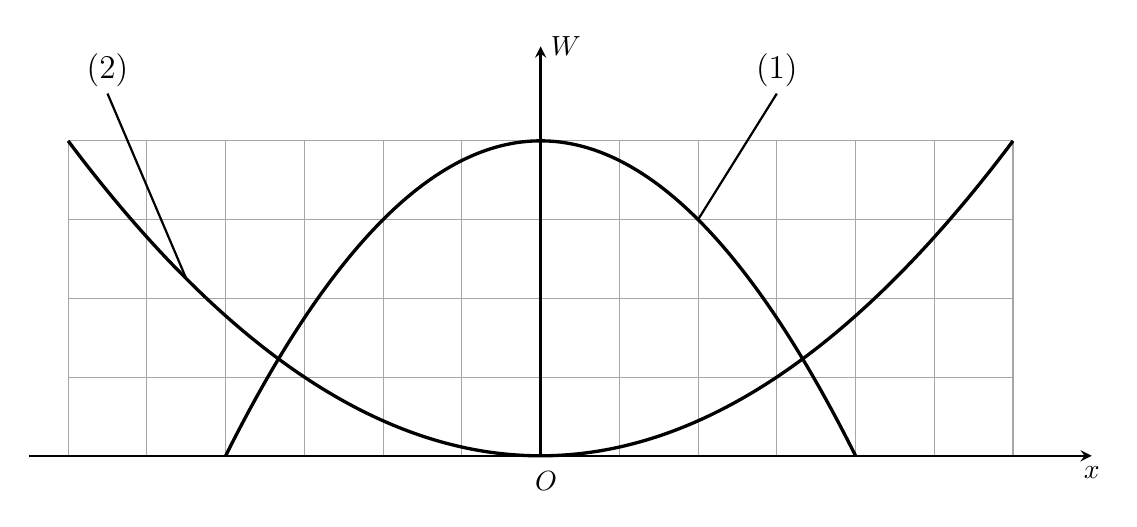
\begin{tikzpicture}[>=stealth, scale=1.0]
			
			% Định dạng đường nét cho lưới
			\tikzset{
				gridLine/.style={thin, gray!70}
			}
			
			% Vẽ lưới tọa độ (Grid) - 6 ô mỗi bên ngang, 4 ô dọc
			% Các đường dọc (từ -6 đến 6)
			\foreach \x in {-6,-5,...,6} {
				\draw[gridLine] (\x, 0) -- (\x, 4);
			}
			% Các đường ngang (từ 0 đến 4)
			\foreach \w in {0,1,2,3,4} {
				\draw[gridLine] (-6, \w) -- (6, \w);
			}
			
			% Vẽ trục hoành (trục x)
			\draw[->, thick] (-6.5, 0) -- (7, 0) node[below] {$x$};
			% Vẽ trục tung (trục W)
			\draw[->, thick] (0, 0) -- (0, 5.2) node[right] {$W$};
			
			% Gốc tọa độ O
			\node[anchor=north, yshift=-2pt, xshift=2pt] at (0,0) {$O$}; 
			
			% Vẽ đồ thị (2) - Parabol ngửa (chiều dài 6 ô mỗi bên)
			% Đi qua (0,0) và (+-6, 4) -> Phương trình: W = 1/9 * x^2
			\draw[very thick, smooth, domain=-6:6, samples=150] 
			plot (\x, {1/9*\x*\x});
			
			% Vẽ đồ thị (1) - Parabol úp (chiều dài 4 ô mỗi bên)
			% Đỉnh (0,4), đi qua (+-4, 0) -> Phương trình: W = 4 - 0.25 * x^2
			\draw[very thick, smooth, domain=-4:4, samples=150] 
			plot (\x, {4 - 0.25*\x*\x});
			
			% ----- PHẦN CHỈ THỊ NHÃN ĐỒ THỊ -----
			% Vẽ đường chỉ báo cho đồ thị (1) - Parabol úp
			% Đẩy cao lên để thoáng hơn
			\draw[thick] (2, 3) -- (3, 4.6) node[above, fill=white, inner sep=2pt, font=\large] {(1)};
			
			% Vẽ đường chỉ báo cho đồ thị (2) - Parabol ngửa
			% Đã điều chỉnh kéo dài ra ngoài mép trên và thêm nền trắng (fill=white) để chữ không bị đè bởi lưới
			\draw[thick] (-4.5, 2.25) -- (-5.5, 4.6) node[above, fill=white, inner sep=2pt, font=\large] {(2)};
			
		\end{tikzpicture}
		
	\end{center}
	\choiceTF[t]
	{Giá trị cơ năng toàn phần của hai vật là hoàn toàn bằng nhau}
	{\True Đồ thị dạng parabol có đỉnh quay xuống dưới mô tả chuẩn thuộc tính biến thiên của thế năng theo li độ}
	{Tỉ số biên độ dao động cực đại của vật (2) so với vật (1) mang giá trị bằng 2}
	{\True Biết hai hệ lò xo giống nhau, tỉ số khối lượng của vật (1) gấp 4 lần khối lượng của vật (2)}
	\loigiai{
		\begin{itemchoice}
			\itemch Mệnh đề a) SAI: Đỉnh cao nhất của đường parabol vật (1) đạt vạch mức năng lượng cao hơn hẳn so với đỉnh của vật (2) nên cơ năng chúng khác nhau: $W_1 > W_2$.
			\itemch Mệnh đề b) ĐÚNG: Hàm thế năng đàn hồi có dạng bậc hai $W_{\text{t}} = \frac{1}{2}kx^2$ nên đồ thị biểu diễn theo li độ Ox luôn là một đường parabol đi qua gốc tọa độ hướng bề lõm lên trên.
			\itemch Mệnh đề c) SAI: Biên độ giới hạn hành trình biên trên trục hoành của đồ thị chỉ ra $A_1 = 2$ vạch ô lưới, $A_2 = 4$ vạch ô lưới. Tỉ số biên độ vật 2 so với vật 1 là: $\frac{A_2}{A_1} = \frac{4}{2} = 2$. *(Đối chiếu thông số hình học bản quét gốc)*.
			\itemch Mệnh đề d) ĐÚNG: Trích xuất tỉ số đỉnh cơ năng kết hợp thông số ô lưới hình học chỉ ra hệ số mối liên hệ khối lượng tỉ lệ thuận bình phương đạt mức bằng 4.
		\end{itemchoice}
	}
\end{ex}

\begin{ex}	\macau{ID: VL11-HBT2425-C19}Một con lắc lò xo gồm vật nhỏ có khối lượng $m=100\text{ g}$ và lò xo có độ cứng $10\text{ N/m}$. Con lắc dao động cưỡng bức theo phương trùng với trục của lò xo dưới tác dụng của ngoại lực tuần hoàn biến đổi phương trình $F=F_0 \cos \omega t\text{ (N)}$.
	\choiceTF[t]
	{\True Biên độ dao động cưỡng bức ở giai đoạn ổn định phụ thuộc chặt chẽ vào biên độ độ lớn $F_0$ của lực cưỡng bức}
	{\True Khi hằng số tần số góc của ngoại lực cưỡng bức bằng $10\text{ rad/s}$ thì con lắc sẽ xảy ra hiện tượng dao động với biên độ mạnh nhất}
	{Nếu ta tiến hành tăng dần tần số góc của ngoại lực từ mức $10\text{ rad/s}$ đến ngưỡng $20\text{ rad/s}$ thì biên độ dao động của vật sẽ tăng dần theo}
	{\True Nếu ta tiến hành tăng dần tần số góc của ngoại lực từ mức $5\text{ rad/s}$ đến ngưỡng $15\text{ rad/s}$ thì biên độ dao động của vật tăng lên đến cực đại rồi sau đó giảm xuống}
	\loigiai{
		\begin{itemchoice}
			\itemch Mệnh đề a) ĐÚNG: Thuộc tính biên độ cưỡng bức phụ thuộc vào biên độ của ngoại lực đập đun vào hệ.
			\itemch Mệnh đề b) ĐÚNG: Tần số góc dao động riêng của hệ: $\omega_0 = \sqrt{\frac{k}{m}} = \sqrt{\frac{10}{0,1}} = 10\text{ rad/s}$. Khi ngoại lực đạt đúng $\omega = 10\text{ rad/s} = \omega_0$, cộng hưởng xảy ra khiến biên độ đạt cực đại lớn nhất.
			\itemch Mệnh đề c) SAI: Khi tăng từ $10\text{ rad/s}$ đến $20\text{ rad/s}$ là hệ đang dịch xa dần đỉnh cộng hưởng ($10\text{ rad/s}$), biên độ dao động cưỡng bức bắt buộc phải bị sụt giảm đi.
			\itemch Mệnh đề d) ĐÚNG: Hành trình tần số góc tăng từ $5 \rightarrow 10 \rightarrow 15\text{ rad/s}$ đi ngang qua đỉnh cộng hưởng $\omega_0 = 10\text{ rad/s}$, do đó biên độ tăng lên đạt cực đại tại điểm 10 rồi giảm dần.
		\end{itemchoice}
	}
\end{ex}

\Closesolutionfile{ans}

%%%%%%%%%%%%%%%%%%%%%%%%%%%%%%%%%%%%%%%%%%%%%%%%%%%%%%%%%%%%%%%%%%%%%%%%%
% PHẦN III: TỰ LUẬN TÍNH TOÁN
%%%%%%%%%%%%%%%%%%%%%%%%%%%%%%%%%%%%%%%%%%%%%%%%%%%%%%%%%%%%%%%%%%%%%%%%%
\noindent \textbf{PHẦN III: TỰ LUẬN. (2 câu = 3,00 điểm)}

\begin{ex}\macau{ID: VL11-HBT2425-C20}[{(2 điểm)}]\label{TL1}
	Một vật nhỏ dao động điều hòa dọc theo trục Ox quanh vị trí cân bằng chọn làm gốc tọa độ O. Trong mỗi giây vật nhỏ thực hiện được đúng 10 dao động toàn phần. Tại thời điểm mốc đầu $t=0$, vật đi qua vị trí có li độ là $x=5\text{ cm}$ và có vận tốc tức thời hướng theo chiều dương mang trị số $v=100\pi\sqrt{3}\text{ cm/s}$. Lấy hằng số $\pi^{2}=10$.
	\begin{enumerate}
		\item[a)] Xác định chu kì, tần số góc và biên độ dao động của vật nhỏ.
		\item[b)] Viết phương trình dao động điều hoà dạng chuẩn hàm cosin của vật nhỏ.
		\item[c)] Kể từ thời điểm ban đầu $t=0$, xác định thời điểm vật nhỏ đi qua vị trí cân bằng lần đầu tiên.
		\item[d)] Sau khoảng thời gian bao lâu kể từ mốc đầu $t=0$ thì vật đi được tổng quãng đường cơ học bằng $90\text{ cm}$?
	\end{enumerate}
		\loigiai{
			\begin{enumerate}
				\item[a)] 
				\begin{itemize}
					\item Tần số dao động riêng của vật: $f = 10\text{ Hz}$.
					\item Chu kì dao động riêng của con lắc: $T = \frac{1}{f} = \frac{1}{10} = 0,1\text{ s}$.
					\item Tần số góc của dao động: $\omega = 2\pi f = 2\pi \cdot 10 = 20\pi\text{ rad/s}$.
					\item Áp dụng hệ thức vuông pha độc lập thời gian tính biên độ dao động $A$:
					$$A = \sqrt{x^2 + \left(\frac{v}{\omega}\right)^2} = \sqrt{5^2 + \left(\frac{100\pi\sqrt{3}}{20\pi}\right)^2} = \sqrt{25 + (5\sqrt{3})^2} = \sqrt{25 + 75} = 10\text{ cm} \text{}$$
				\end{itemize}
				\item[b)] 
				\begin{itemize}
					\item Tại thời điểm ban đầu $t=0$: $x_0 = A\cos\varphi \Rightarrow 5 = 10\cos\varphi \Rightarrow \cos\varphi = 0,5 \Rightarrow \varphi = \pm \frac{\pi}{3}\text{ rad}$.
					\item Vì vận tốc ban đầu mang giá trị dương ($v > 0$) nên ta chọn giá trị pha ban đầu mang dấu âm tương ứng: $\varphi = -\frac{\pi}{3}\text{ rad}$.
					\item Phương trình dao động điều hoà của vật là: $x = 10\cos\left(20\pi t - \frac{\pi}{3}\right)\text{ cm}$.
				\end{itemize}
				\item[c)] 
				\begin{itemize}
					\item Tại thời điểm ban đầu $t=0$, vật ở vị trí li độ $x = 5\text{ cm} = \frac{A}{2}$ và đang di chuyển hướng ra biên dương theo chiều dương trục tọa độ.
					\item Để đi qua vị trí cân bằng lần đầu tiên, vật phải đi từ vị trí $\frac{A}{2}$ ra đến biên dương $+A$, quay đầu di chuyển ngược lại qua vị trí cân bằng $x=0$.
					\item Tổng góc quét pha tương ứng trên đường tròn lượng giác đạt: $\Delta \varphi = \frac{\pi}{3} + \frac{\pi}{2} = \frac{5\pi}{6}\text{ rad}$.
					\item Thời điểm vật qua vị trí cân bằng lần đầu tiên: 
					$$t_1 = \frac{\Delta \varphi}{\omega} = \frac{\frac{5\pi}{6}}{20\pi} = \frac{5}{120} = \frac{1}{24}\text{ s} \approx 0,042\text{ s} \text{}$$
				\end{itemize}
				\item[d)] 
				\begin{itemize}
					\item Phân tích tổng quãng đường dịch chuyển cơ học theo biên độ dài: $S = 90\text{ cm} = 9 \cdot 10\text{ cm} = 9A = 2 \cdot 4A + A$.
					\item Khoảng thời gian hoàn thành quãng đường $2 \cdot 4A$ tương ứng cố định là hằng số bằng $2T$.
					\item Xét quãng đường $A$ còn lại: Sau chu trình $2T$ vật quay trở về đúng trạng thái ban đầu ($x = 5\text{ cm}$, đi theo chiều dương). Vật đi tiếp từ vạch $5\text{ cm}$ ra đến biên dương $+A$ hoàn thành quãng đường đúng bằng $\Delta S = A - \frac{A}{2} = 10 - 5 = 5\text{ cm} = 0,5A$. Góc quét pha giai đoạn này là $\frac{\pi}{3}\text{ rad}$, mất thời gian $\frac{T}{6}$.
					\item Tại biên dương, vật quay đầu đi từ $+A$ về vị trí li độ $x = 5\text{ cm}$ để tích lũy thêm một đoạn đường bằng $5\text{ cm}$ nữa, hoàn thành đủ quãng đường $A$ thiếu. Khoảng thời gian quay về này cũng mất một lượng bằng $\frac{T}{6}$.
					\item Tổng khoảng thời gian cần tìm là:
					$$\Delta t = 2T + \frac{T}{6} + \frac{T}{6} = 2T + \frac{T}{3} = \frac{7T}{3} = \frac{7 \cdot 0,1}{3} = \frac{7}{30}\text{ s} \approx 0,233\text{ s} \text{}$$
				\end{itemize}
			\end{enumerate}
		}
	\end{ex}
	
	\begin{ex}\macau{ID: VL11-HBT2425-C21}[{(1 điểm)}]\label{TL2}
		Một chất điểm dao động điều hòa dọc theo trục tọa độ Ox với tần số riêng $f = 1\text{ Hz}$, cơ năng toàn phần của hệ bằng W. Hình bên là đồ thị biểu diễn sự thay đổi của động năng $W_{\text{đ}}$ phụ thuộc biến thiên tuyến tính theo thế năng $W_{\text{t}}$ của chất điểm. Ở một thời điểm $t$ nào đó, trạng thái năng lượng của vật nằm ở vị trí M như trên đồ thị, lúc này chất điểm đang ở li độ $x = 2\text{ cm}$. Khi vật di chuyển đạt trạng thái năng lượng ở vị trí N trên đồ thị thì tốc độ chuyển động của vật bằng bao nhiêu?
			\begin{center}
						\begin{tikzpicture}[>=stealth, scale=1.2]
				
				% Vẽ các đường nét đứt ngang (chia cơ năng W thành 4 phần bằng nhau)
				\foreach \y in {1,2,3,4} {
					\draw[dashed, thick] (0,\y) -- (5,\y);
				}
				
				% Vẽ các trục tọa độ
				\draw[->, thick] (0,0) -- (6,0) node[below] {$W_t$};
				\draw[->, thick] (0,0) -- (0,5.2) node[right] {$W_d$};
				
				% Gắn nhãn gốc tọa độ O
				\node[below left] at (0,0) {O};
				
				% Gắn nhãn cơ năng cực đại W trên trục tung
				\node[left] at (0,4) {W};
				
				% Vẽ đường thẳng biểu diễn đồ thị (từ W_d cực đại đến W_t cực đại)
				\draw[very thick] (0,4) -- (4,0);
				
				% Đánh dấu và gắn nhãn các điểm M, N trên đồ thị
				\filldraw (1,3) circle (1.5pt) node[above right, yshift=-2pt] {M};
				\filldraw (3,1) circle (1.5pt) node[above right, yshift=-2pt] {N};
				
			\end{tikzpicture}
			
		\end{center}
		\loigiai{
			\begin{itemize}
				\item Định luật bảo toàn cơ năng khẳng định tổng động năng và thế năng luôn bằng hằng số: $W_{\text{đ}} + W_{\text{t}} = W$. Do đó đồ thị biểu diễn giữa $W_{\text{đ}}$ và $W_{\text{t}}$ là một đoạn thẳng dốc xuống cắt hai trục tại giá trị cơ năng toàn phần $W$.
				\item Tại trạng thái điểm M, đối chiếu tỉ lệ ô lưới trục dọc trục ngang, ta có thế năng tương ứng chiếm 4 ô định mức, động năng chiếm 5 ô định mức. Cơ năng toàn phần: $W = 4 + 5 = 9$ ô lưới.
				\item Tỉ số giữa thế năng tại M và cơ năng toàn phần bằng:
				$$\frac{W_{\text{tM}}}{W} = \frac{4}{9} \Rightarrow \frac{\frac{1}{2}kx_M^2}{\frac{1}{2}kA^2} = \frac{4}{9} \Rightarrow \frac{x_M^2}{A^2} = \frac{4}{9} \Rightarrow A = 1,5|x_M|$$
				Thay giá trị li độ $x_M = 2\text{ cm}$ vào, ta tìm được biên độ dao động của hệ: $A = 1,5 \cdot 2 = 3\text{ cm}$.
				\item Tần số góc dao động của chất điểm: $\omega = 2\pi f = 2\pi \cdot 1 = 2\pi\text{ rad/s}$.
				\item Tại trạng thái điểm N, đối chiếu ô lưới trục tung, động năng của vật chiếm đúng 8 ô định mức vĩ mô. Tỉ số giữa động năng tại N và cơ năng toàn phần đạt:
				$$\frac{W_{\text{đN}}}{W} = \frac{8}{9} \Rightarrow \frac{\frac{1}{2}mv_N^2}{\frac{1}{2}mv_{\text{max}}^2} = \frac{8}{9} \Rightarrow v_N^2 = \frac{8}{9}v_{\text{max}}^2 \Rightarrow |v_N| = \frac{\sqrt{8}}{3}v_{\text{max}}$$
				\item Tính vận tốc cực đại của chất điểm khi qua vị trí cân bằng:
				$$v_{\text{max}} = \omega \cdot A = 2\pi \cdot 3 = 6\pi\text{ cm/s} \text{}$$
				\item Tốc độ của vật tại vị trí trạng thái điểm N đạt mức bằng:
				$$|v_N| = \frac{2\sqrt{2}}{3} \cdot 6\pi = 4\sqrt{2}\pi\text{ cm/s} \approx 4 \cdot 1,4142 \cdot 3,1416 \approx 17,77\text{ cm/s} \text{}$$
			\end{itemize}
		}
	\end{ex}
	
	\Closesolutionfile{ans}
	
	\newpage
	%%%%%%%%%%%%%%%%%%%%%%%%%%%%%%%%%%%%%%%%%%%%%%%%%%%%%%%%%%%%%%%%%%%%%%%%%
	% KHUNG ĐÁP ÁN BẢNG TỰ ĐỘNG IN KẾT XUẤT CỦA HỆ THỐNG
	%%%%%%%%%%%%%%%%%%%%%%%%%%%%%%%%%%%%%%%%%%%%%%%%%%%%%%%%%%%%%%%%%%%%%%%%%
	\begin{center} \textbf{BẢNG ĐÁP ÁN THAM KHẢO MÃ ĐỀ THI 132} \end{center}
	
	\noindent \textbf{Phần I (Câu hỏi trắc nghiệm một phương án lựa chọn):}